
%% bare_conf.tex
%% V1.3
%% 2007/01/11
%% by Michael Shell
%% See:
%% http://www.michaelshell.org/
%% for current contact information.
%%
%% This is a skeleton file demonstrating the use of IEEEtran.cls
%% (requires IEEEtran.cls version 1.7 or later) with an IEEE conference paper.
%%
%% Support sites:
%% http://www.michaelshell.org/tex/ieeetran/
%% http://www.ctan.org/tex-archive/macros/latex/contrib/IEEEtran/
%% andd
%% http://www.ieee.org/

%%*************************************************************************
%% Legal Notice:
%% This code is offered as-is without any warranty either expressed or
%% implied; without even the implied warranty of MERCHANTABILITY or
%% FITNESS FOR A PARTICULAR PURPOSE! 
%% User assumes all risk.
%% In no event shall IEEE or any contributor to this code be liable for
%% any damages or losses, including, but not limited to, incidental,
%% consequential, or any other damages, resulting from the use or misuse
%% of any information contained here.
%%
%% All comments are the opinions of their respective authors and are not
%% necessarily endorsed by the IEEE.
%%
%% This work is distributed under the LaTeX Project Public License (LPPL)
%% ( http://www.latex-project.org/ ) version 1.3, and may be freely used,
%% distributed and modified. A copy of the LPPL, version 1.3, is included
%% in the base LaTeX documentation of all distributions of LaTeX released
%% 2003/12/01 or later.
%% Retain all contribution notices and credits.
%% ** Modified files should be clearly indicated as such, including  **
%% ** renaming them and changing author support contact information. **
%%
%% File list of work: IEEEtran.cls, IEEEtran_HOWTO.pdf, bare_adv.tex,
%%                    bare_conf.tex, bare_jrnl.tex, bare_jrnl_compsoc.tex
%%*************************************************************************

% *** Authors should verify (and, if needed, correct) their LaTeX system  ***
% *** with the testflow diagnostic prior to trusting their LaTeX platform ***
% *** with production work. IEEE's font choices can trigger bugs that do  ***
% *** not appear when using other class files.                            ***
% The testflow support page is at:
% http://www.michaelshell.org/tex/testflow/



% Note that the a4paper option is mainly intended so that authors in
% countries using A4 can easily print to A4 and see how their papers will
% look in print - the typesetting of the document will not typically be
% affected with changes in paper size (but the bottom and side margins will).
% Use the testflow package mentioned above to verify correct handling of
% both paper sizes by the user's LaTeX system.
%
% Also note that the "draftcls" or "draftclsnofoot", not "draft", option
% should be used if it is desired that the figures are to be displayed in
% draft mode.
%
\documentclass[conference]{IEEEtran}
\IEEEoverridecommandlockouts
\linespread{0.85}
% Add the compsoc option for Computer Society conferences.
%
% If IEEEtran.cls has not been installed into the LaTeX system files,
% manually specify the path to it like:
% \documentclass[conference]{../sty/IEEEtran}





% Some very useful LaTeX packages include:
% (uncomment the ones you want to load)


% *** MISC UTILITY PACKAGES ***
%
%\usepackage{ifpdf}
% Heiko Oberdiek's ifpdf.sty is very useful if you need conditional
% compilation based on whether the output is pdf or dvi.
% usage:
% \ifpdf
%   % pdf code
% \else
%   % dvi code
% \fi
% The latest version of ifpdf.sty can be obtained from:
% http://www.ctan.org/tex-archive/macros/latex/contrib/oberdiek/
% Also, note that IEEEtran.cls V1.7 and later provides a builtin
% \ifCLASSINFOpdf conditional that works the same way.
% When switching from latex to pdflatex and vice-versa, the compiler may
% have to be run twice to clear warning/error messages.






% *** CITATION PACKAGES ***
%
%\usepackage{cite}
% cite.sty was written by Donald Arseneau
% V1.6 and later of IEEEtran pre-defines the format of the cite.sty package
% \cite{} output to follow that of IEEE. Loading the cite package will
% result in citation numbers being automatically sorted and properly
% "compressed/ranged". e.g., [1], [9], [2], [7], [5], [6] without using
% cite.sty will become [1], [2], [5]--[7], [9] using cite.sty. cite.sty's
% \cite will automatically add leading space, if needed. Use cite.sty's
% noadjust option (cite.sty V3.8 and later) if you want to turn this off.
% cite.sty is already installed on most LaTeX systems. Be sure and use
% version 4.0 (2003-05-27) and later if using hyperref.sty. cite.sty does
% not currently provide for hyperlinked citations.
% The latest version can be obtained at:
% http://www.ctan.org/tex-archive/macros/latex/contrib/cite/
% The documentation is contained in the cite.sty file itself.






% *** GRAPHICS RELATED PACKAGES ***
%
\ifCLASSINFOpdf
  \usepackage[pdftex]{graphicx}
  % declare the path(s) where your graphic files are
  % \graphicspath{{../pdf/}{../jpeg/}}
  % and their extensions so you won't have to specify these with
  % every instance of \includegraphics
  % \DeclareGraphicsExtensions{.pdf,.jpeg,.png}
\else
  % or other class option (dvipsone, dvipdf, if not using dvips). graphicx
  % will default to the driver specified in the system graphics.cfg if no
  % driver is specified.
  % \usepackage[dvips]{graphicx}
  % declare the path(s) where your graphic files are
  % \graphicspath{{../eps/}}
  % and their extensions so you won't have to specify these with
  % every instance of \includegraphics
  % \DeclareGraphicsExtensions{.eps}
\fi
% graphicx was written by David Carlisle and Sebastian Rahtz. It is
% required if you want graphics, photos, etc. graphicx.sty is already
% installed on most LaTeX systems. The latest version and documentation can
% be obtained at: 
% http://www.ctan.org/tex-archive/macros/latex/required/graphics/
% Another good source of documentation is "Using Imported Graphics in
% LaTeX2e" by Keith Reckdahl which can be found as epslatex.ps or
% epslatex.pdf at: http://www.ctan.org/tex-archive/info/
%
% latex, and pdflatex in dvi mode, support graphics in encapsulated
% postscript (.eps) format. pdflatex in pdf mode supports graphics
% in .pdf, .jpeg, .png and .mps (metapost) formats. Users should ensure
% that all non-photo figures use a vector format (.eps, .pdf, .mps) and
% not a bitmapped formats (.jpeg, .png). IEEE frowns on bitmapped formats
% which can result in "jaggedy"/blurry rendering of lines and letters as
% well as large increases in file sizes.
%
% You can find documentation about the pdfTeX application at:
% http://www.tug.org/applications/pdftex





% *** MATH PACKAGES ***
%
%\usepackage[cmex10]{amsmath}
% A popular package from the American Mathematical Society that provides
% many useful and powerful commands for dealing with mathematics. If using
% it, be sure to load this package with the cmex10 option to ensure that
% only type 1 fonts will utilized at all point sizes. Without this option,
% it is possible that some math symbols, particularly those within
% footnotes, will be rendered in bitmap form which will result in a
% document that can not be IEEE Xplore compliant!
%
% Also, note that the amsmath package sets \interdisplaylinepenalty to 10000
% thus preventing page breaks from occurring within multiline equations. Use:
%\interdisplaylinepenalty=2500
% after loading amsmath to restore such page breaks as IEEEtran.cls normally
% does. amsmath.sty is already installed on most LaTeX systems. The latest
% version and documentation can be obtained at:
% http://www.ctan.org/tex-archive/macros/latex/required/amslatex/math/





% *** SPECIALIZED LIST PACKAGES ***
%
%\usepackage{algorithmic}
% algorithmic.sty was written by Peter Williams and Rogerio Brito.
% This package provides an algorithmic environment fo describing algorithms.
% You can use the algorithmic environment in-text or within a figure
% environment to provide for a floating algorithm. Do NOT use the algorithm
% floating environment provided by algorithm.sty (by the same authors) or
% algorithm2e.sty (by Christophe Fiorio) as IEEE does not use dedicated
% algorithm float types and packages that provide these will not provide
% correct IEEE style captions. The latest version and documentation of
% algorithmic.sty can be obtained at:
% http://www.ctan.org/tex-archive/macros/latex/contrib/algorithms/
% There is also a support site at:
% http://algorithms.berlios.de/index.html
% Also of interest may be the (relatively newer and more customizable)
% algorithmicx.sty package by Szasz Janos:
% http://www.ctan.org/tex-archive/macros/latex/contrib/algorithmicx/




% *** ALIGNMENT PACKAGES ***
%
%\usepackage{array}
% Frank Mittelbach's and David Carlisle's array.sty patches and improves
% the standard LaTeX2e array and tabular environments to provide better
% appearance and additional user controls. As the default LaTeX2e table
% generation code is lacking to the point of almost being broken with
% respect to the quality of the end results, all users are strongly
% advised to use an enhanced (at the very least that provided by array.sty)
% set of table tools. array.sty is already installed on most systems. The
% latest version and documentation can be obtained at:
% http://www.ctan.org/tex-archive/macros/latex/required/tools/


%\usepackage{mdwmath}
%\usepackage{mdwtab}
% Also highly recommended is Mark Wooding's extremely powerful MDW tools,
% especially mdwmath.sty and mdwtab.sty which are used to format equations
% and tables, respectively. The MDWtools set is already installed on most
% LaTeX systems. The lastest version and documentation is available at:
% http://www.ctan.org/tex-archive/macros/latex/contrib/mdwtools/


% IEEEtran contains the IEEEeqnarray family of commands that can be used to
% generate multiline equations as well as matrices, tables, etc., of high
% quality.


%\usepackage{eqparbox}
% Also of notable interest is Scott Pakin's eqparbox package for creating
% (automatically sized) equal width boxes - aka "natural width parboxes".
% Available at:
% http://www.ctan.org/tex-archive/macros/latex/contrib/eqparbox/





% *** SUBFIGURE PACKAGES ***
%\usepackage[tight,footnotesize]{subfigure}
% subfigure.sty was written by Steven Douglas Cochran. This package makes it
% easy to put subfigures in your figures. e.g., "Figure 1a and 1b". For IEEE
% work, it is a good idea to load it with the tight package option to reduce
% the amount of white space around the subfigures. subfigure.sty is already
% installed on most LaTeX systems. The latest version and documentation can
% be obtained at:
% http://www.ctan.org/tex-archive/obsolete/macros/latex/contrib/subfigure/
% subfigure.sty has been superceeded by subfig.sty.



%\usepackage[caption=false]{caption}
%\usepackage[font=footnotesize]{subfig}
% subfig.sty, also written by Steven Douglas Cochran, is the modern
% replacement for subfigure.sty. However, subfig.sty requires and
% automatically loads Axel Sommerfeldt's caption.sty which will override
% IEEEtran.cls handling of captions and this will result in nonIEEE style
% figure/table captions. To prevent this problem, be sure and preload
% caption.sty with its "caption=false" package option. This is will preserve
% IEEEtran.cls handing of captions. Version 1.3 (2005/06/28) and later 
% (recommended due to many improvements over 1.2) of subfig.sty supports
% the caption=false option directly:
%\usepackage[caption=false,font=footnotesize]{subfig}
%
% The latest version and documentation can be obtained at:
% http://www.ctan.org/tex-archive/macros/latex/contrib/subfig/
% The latest version and documentation of caption.sty can be obtained at:
% http://www.ctan.org/tex-archive/macros/latex/contrib/caption/




% *** FLOAT PACKAGES ***
%
%\usepackage{fixltx2e}
% fixltx2e, the successor to the earlier fix2col.sty, was written by
% Frank Mittelbach and David Carlisle. This package corrects a few problems
% in the LaTeX2e kernel, the most notable of which is that in current
% LaTeX2e releases, the ordering of single and double column floats is not
% guaranteed to be preserved. Thus, an unpatched LaTeX2e can allow a
% single column figure to be placed prior to an earlier double column
% figure. The latest version and documentation can be found at:
% http://www.ctan.org/tex-archive/macros/latex/base/



%\usepackage{stfloats}
% stfloats.sty was written by Sigitas Tolusis. This package gives LaTeX2e
% the ability to do double column floats at the bottom of the page as well
% as the top. (e.g., "\begin{figure*}[!b]" is not normally possible in
% LaTeX2e). It also provides a command:
%\fnbelowfloat
% to enable the placement of footnotes below bottom floats (the standard
% LaTeX2e kernel puts them above bottom floats). This is an invasive package
% which rewrites many portions of the LaTeX2e float routines. It may not work
% with other packages that modify the LaTeX2e float routines. The latest
% version and documentation can be obtained at:
% http://www.ctan.org/tex-archive/macros/latex/contrib/sttools/
% Documentation is contained in the stfloats.sty comments as well as in the
% presfull.pdf file. Do not use the stfloats baselinefloat ability as IEEE
% does not allow \baselineskip to stretch. Authors submitting work to the
% IEEE should note that IEEE rarely uses double column equations and
% that authors should try to avoid such use. Do not be tempted to use the
% cuted.sty or midfloat.sty packages (also by Sigitas Tolusis) as IEEE does
% not format its papers in such ways.





% *** PDF, URL AND HYPERLINK PACKAGES ***
%
%\usepackage{url}
% url.sty was written by Donald Arseneau. It provides better support for
% handling and breaking URLs. url.sty is already installed on most LaTeX
% systems. The latest version can be obtained at:
% http://www.ctan.org/tex-archive/macros/latex/contrib/misc/
% Read the url.sty source comments for usage information. Basically,
% \url{my_url_here}.





% *** Do not adjust lengths that control margins, column widths, etc. ***
% *** Do not use packages that alter fonts (such as pslatex).         ***
% There should be no need to do such things with IEEEtran.cls V1.6 and later.
% (Unless specifically asked to do so by the journal or conference you plan
% to submit to, of course. )

%\usepackage[margin=0.75in]{geometry}
%%\usepackage[hmargin=0.75in,vmargin=1.0in]{geometry}
% correct bad hyphenation here
\hyphenation{op-tical net-works semi-conduc-tor}

\setlength{\abovecaptionskip}{-1pt}
%\setlength{\belowcaptionskip}{-200pt}
%\setlength{\intextsep}{-1mm}
\begin{document}

%
% paper title
% can use linebreaks \\ within to get better formatting as desired
%\title{Adult-Size Humanoid Robot Throwing the First Pitch at a Major League Baseball Game \\ A Road Map}
\title{Humanoid Pitching at a Major League Baseball Game: Challenges, Approach, Implementation and Lessons Learned}

% author names and affiliations
% use a multiple column layout for up to three different
% affiliations
\author{\IEEEauthorblockN{Daniel M. Lofaro}
\IEEEauthorblockA{Electrical and Computer Engineering\\
Drexel University\\
Philadelphia, PA, USA\\
Email: dan@danLofaro.com}
\and
\IEEEauthorblockN{Sun Chunyang}
\IEEEauthorblockA{Mechanical Engineering\\
Nanyang Technological University\\
Singapore\\
Email: sunc0012@e.ntu.edu.sg}
\and
\IEEEauthorblockN{Paul Oh}
\IEEEauthorblockA{Mechanical Engineering\\
Drexel University\\
Philadelphia, PA, USA\\
Email: paul@coe.drexel.edu}
\thanks{\bf{*This project was supported by a Partnerships for International Research and Education (PIRE) \#0730206, and Major Research Infrastructure Recovery and Reinvestment (MIRR) \#CNS-0960061 sponsored by the the U.S. National Science Foundation (NSF).}}
}





% conference papers do not typically use \thanks and this command
% is locked out in conference mode. If really needed, such as for
% the acknowledgment of grants, issue a \IEEEoverridecommandlockouts
% after \documentclass

% for over three affiliations, or if they all won't fit within the width
% of the page, use this alternative format:
% 
%\author{\IEEEauthorblockN{Michael Shell\IEEEauthorrefmark{1},
%Homer Simpson\IEEEauthorrefmark{2},
%James Kirk\IEEEauthorrefmark{3}, 
%Montgomery Scott\IEEEauthorrefmark{3} and
%Eldon Tyrell\IEEEauthorrefmark{4}}
%\IEEEauthorblockA{\IEEEauthorrefmark{1}School of Electrical and Computer Engineering\\
%Georgia Institute of Technology,
%Atlanta, Georgia 30332--0250\\ Email: see http://www.michaelshell.org/contact.html}
%\IEEEauthorblockA{\IEEEauthorrefmark{2}Twentieth Century Fox, Springfield, USA\\
%Email: homer@thesimpsons.com}
%\IEEEauthorblockA{\IEEEauthorrefmark{3}Starfleet Academy, San Francisco, California 96678-2391\\
%Telephone: (800) 555--1212, Fax: (888) 555--1212}
%\IEEEauthorblockA{\IEEEauthorrefmark{4}Tyrell Inc., 123 Replicant Street, Los Angeles, California 90210--4321}}




% use for special paper notices
%\IEEEspecialpapernotice{(Invited Paper)}




% make the title area
\maketitle


\begin{abstract}
%\boldmath
\begin{center}
\large\bf{Abstract:}
\end{center}
\normalsize

\bf{
\noindent The degrees of freedom (DOF) of robots and complex systems have been increasing increasing exponentially since the early 20th century.
Today it is common place for complex control systems to have 40 DOF. 
This number is projected to be 70 DOF by the year 2020.
Robots with high DOF allows for complex tasks such as tool manipulation, greater human-robot interaction and agile full-body locomotion.
More DOF require greater attention to local communication delays, bandwidth, system configuration and stability.
In addition different tasks being performed by separate parts of the robot in tandem bring on greater issues including controller timing and priorities.
The increase in DOF on single system requires that the traditional methods of controller design be re-examined.

\noindent This dissertation describes a Unified Algorithmic Framework for High Degree of Freedom Complex Systems and Humanoid Robots that allows a user to develop controllers using a three tier infrastructure.
The Unified Algorithmic Framework called Hubo-Ach is a multi-process based system that allows for robust multi-rate simultaneous control and seamless implementation between virtual, miniature, and full-size robots with no modification.
The three tier infrastructure provides different levels of cost to entry and testing.
Examples of this field tested framework functioning on simulated, miniature, and full-size high DOF robots is given as well as validation by external researchers.
}




\end{abstract}
% IEEEtran.cls defaults to using nonbold math in the Abstract.
% This preserves the distinction between vectors and scalars. However,
% if the conference you are submitting to favors bold math in the abstract,
% then you can use LaTeX's standard command \boldmath at the very start
% of the abstract to achieve this. Many IEEE journals/conferences frown on
% math in the abstract anyway.

% no keywords




% For peer review papers, you can put extra information on the cover
% page as needed:
% \ifCLASSOPTIONpeerreview
% \begin{center} \bfseries EDICS Category: 3-BBND \end{center}
% \fi
%
% For peerreview papers, this IEEEtran command inserts a page break and
% creates the second title. It will be ignored for other modes.
\IEEEpeerreviewmaketitle

The number of degrees of freedom (DOF) of control systems are increasing exponentially since the early 20$^{th}$ century.
Today it is common place for complex control systems to have 40 DOF. 
This number is projected to be 70 DOF by the year 2020 (see Section~\ref{sec:numdof}).
\textit{The increase in DOF on single system requires that the traditional methods of controller design needs to be re-examined}.
High DOF complex system, or robots, allow for complex tasks such as using human tools and interfaces \cite{lofaroRAM2013,lofaroTePRA2013HuboAch,lofaroTePRA2013Valve,gtechIK}, playing music \cite{lofaroEURASIP2011, 6094987,lofaroIASTED2011,5686847} and other complex tasks \cite{lofaroHumanoids2012,lofaroGamesRobot,tepraLadder2013}.

\cite{orocos-gadeyne-ijrr2005}
\cite{multiPC-arch-1185243}
\cite{multi-thread-robot-5602743}
\cite{multi-thread-snake-1541141}
\cite{multi-thread-5524083}
\cite{openHRP}
\cite{Webots}




Due to the nature of these highly redundant complex electrical mechanical system it is common to have multiple different controllers running in tandem.  
Different controllers are needed when the system is in different states or doing different tasks or performing multiple tasks at the same time.
Combining these controllers is a problem in complex system.
This problem is hard when each controller has different frequencies, timing requirements (asyncronous vs. syncronous), latency restrictions, newest state data ie smore important then older state data and most basic of all languages the controller is written in.
This is especially true for complete and complex autonomous systems.
I define a complete and complex autonomous system as an electro mechanical mechanism with high degree of freedom (DOF) that is capable of making its own decisions through the use of sensor data processed by its artificial intelligence (AI).
The combination of high DOF and the requirement for autonomy makes the work space broad and controllers complex.
The overarching question becomes; What is the control system structure for a complete and complex autonomous systems with high DOF, a multitude of sensors, AI performing high-level and low-level tasks all while keeping a stable system structure conducive to collaborative work?
Current methods of solving the problem of controller synchrony and latest state data is to keep your critical control elements in the primary control loop.
Inter-process communication (IPC) and/or network sockets to communicate between the high level and low level processes even if written in different languages.
The majority of IPC have the problem of \textit{head of line} blocking (HOL) which means you must read the older data in a buffer before you read the newest data.
In the computer science field this is not a problem because all data being intact is typically desired.  
In the field of robotics and control the most recent state data is more important to a real-time control system to act on.
This thesis shows that by expanding on the idea of multi-process controllers connected to high-speed low-latency IPC you can create a \textit{robot layer} on a computer platform that will allow low-level controllers to run in separate processes while still allowing them access to the most recent data as the priority.
The new technical idea is the \textit{robot layer}, a control layer that allows external processes to run like normal and not deal with the specifics of the given robot system.
The robot system can be replaced by a simulated system without any of the processes needing to be modified or even know of the change.
This allows more mature controllers to be easily interfaced with this system without modifying control rates or timing.
This \textit{robot layer} must be:
\begin{itemize}
\item Have a IPC latency much less then that of the robot's inherent sampling period $t_{ipc}<<T_{r}$
\item Allow for command rates much slower then the inherent sampling period $T_{slow}>>T_{r}$
\item Allow for command rates much faster then the inherent sampling period $T_{fast}<<T_{r}$
\item Allow for arbitrary command rates.
\item Allow for real-time and non-real-time controllers to command actuators
\item Allow for all processes to have access to the newest data first
\item Allow for no more then one rt time step delay between command and robot actuator retrieval
\item Commanded such that it is for an arbitrary robotic actuator.
\item Triggering for process synchronization
\item Triggering for simulator synchronization and holding
\end{itemize}
We can succeed now not only because the bleeding edge technology allows for the fast enough communication between processes with access to the latest data.

Results are measured quantitatively and qualitatively.
Data showing proper loop rates, timings, controller implementation, simulation connections etc. show the viability of the system.
User survey shows methodology is sound, useful, and practical.





My Thesis shows is that a multi-process control structure coupled with the proper timing mechanisms is conducive to answering these questions.
It is shown with physical experiments and the creation of Hubo-Ach\cite{lofaroRAM2013}; a fully functional Sim-Time and Real-Time control system for complete and complex autonomous systems.

Through experimentation I prove my control system is a viable way of controlling complete and complex autonomous system and still be conducive to collaborative work.  
A road map of how my research has taken me to my thesis is shown in Section~\ref{sec:roadmap}.
As proof of viability I show the basic structure of my system \textit{Hubo-Ach} in Section~\ref{sec:hubo-ach}.  
I give step by step examples in Section~\ref{sec:simpleExamples}.
Section~\ref{sec:simulator} shows how we can move from real-time to using a simulated version of the platform in simulation time without having to change the controller.
Section~\ref{sec:task} describes the experiment which consists of making the robot preform an advanced task that pulls together visual, kinematic, path planning and other controllers together using this one system.
The techniques used stem from my contributions in Section~\ref{sec:contributions}.
Section~\ref{sec:results} shows the results of the experiment thus show the viability of the system.
Lastly Section~\ref{sec:conclusion} discusses the results of the work and the future of this system.

Before I continue it is important to note that my work has already been validated by my pears because:
\begin{itemize}
\item It was chosen to be the primary control system for the DARPA Robotics Challenge Track-A Team DRC-Hubo, Section~\ref{sec:drc}.
\item It is being used in the NSF-MIRR project\footnote{NSF-MIRR: Major Research Infrastructure Recovery and Reinvestment (MIRR) \#CNS-0960061 sponsored by the the U.S. National Science Foundation (NSF)}.
\item It is currently being used by MIT, WPI, Purdue, Ohio State, Swarthmore College, Georgia Tech, and Drexel University.
\end{itemize}

For the remainder of this document the complete and complex autonomous systems that I will be referring to are robots.
The majority of examples given will be in reference to humanoid robotics and the Hubo2+ (KHR-4+) platform.
The Hubo platform is described in Section~\ref{sec:hubo}.





The idea for a Control Archetecture for High Degree of Freedom Complex Systems stems from a gap in physical implimentation of control algerithms for robot hardware.

The simplest approach to developing robot software is to intergrate all functionality in one program.  
This functionality includes the following controllers:
\begin{itemize}
\item Hardware Control
\item Perception
\item Planning
\item Kinimatics
\item etc.
\end{itemize}

If all of this functionality is in one process then it has the bennifit of freedom of inter process comunication latency.
However being in one process also means that if one of the controllers laggs or faults it cause the entire controller to lag or fault.
This is of great concern if a non-prority controller such as vision processing faults causing a priority controller such as a ballance controller, to fail.
This will cause the robot to fall.
How is this fixed?
One solution and my proposed solution is to use inter-process comunicatoin (IPC).
Inter-process comunication is a method of exchanging data between multiple processies.
Typical POSIX methods (cite here) give you the \textbf{oldest} information first and have locks on the memroy when processies are writing to it.
Robots work in the physical world. 
More recent information is more important to it then older.
In most cases it is acceptiable to know the most recent data and never read any of the older data.
This would happen if your sensors update at a faster rate then that of the robot.
Typically robot actuiators have a bandwidth much much lower then that of a mondern conputer.
If sensor informatio is shared using traditional shared memory over POSIX methods the controller would have to read the older information before it reaches the information it is most interested in, the newest data.
This is called head of line blocking (look up).

It is desired to make a multi-process controller that can share data between multiple processies with low-latency and no head of line blocking.
There are a few IPCs that offer no head of line blocking and low-latency.  
After much research (inserte examples here) it was found that the Ach IPC wuld best fit my needs.



\section{Methodology}\label{sec:methodology}
%\subsection{Balance and Stability}\label{sec:sec:balance}
Each of the methods used have to be stable through the motion in order for the system to be stable (i.e. not to fall down).  
The well known zero-moment-point (ZMP) criteria is what each method must adhere to in order to stay statically stable\cite{Vukobratovic19721}.  
To handle perturbation an active balance controller was added.  
The active balance controller is applied on top of the pre-defined trajectories.  
Hubo is modeled as a single inverted pendulum with the center of mass (COM) located at length $L$ from the ankle.  
The compliance of the robot is composed of a spring $K$ and a damper $C$, see Fig.~\ref{fig:invPen}.  
An IMU located at the COM gives the measured orientation.

\begin{figure}[t]
  \centering
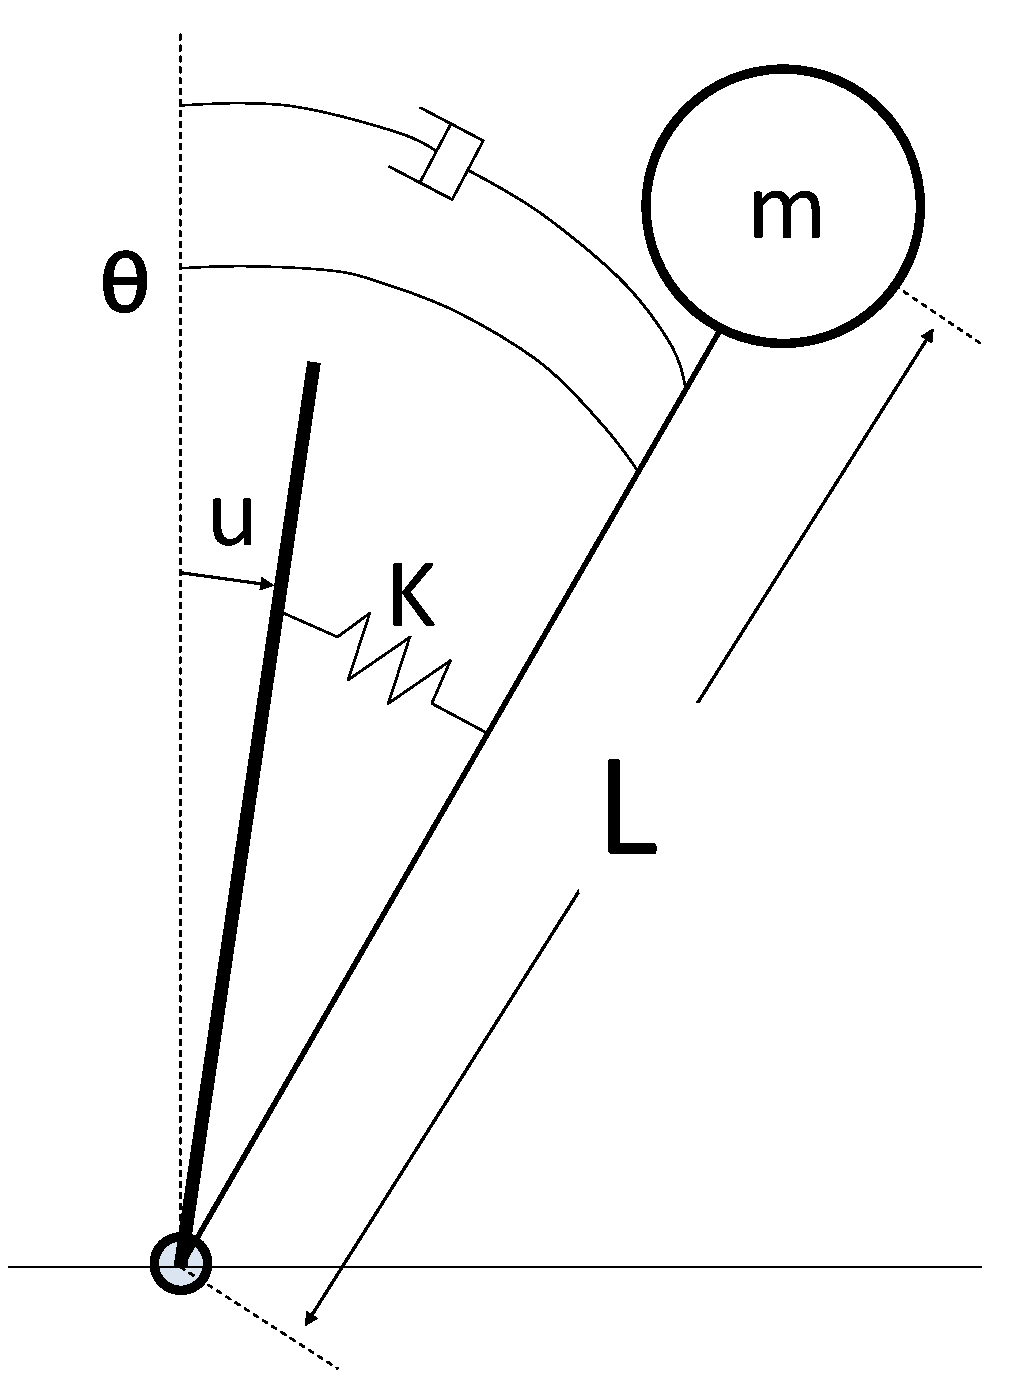
\includegraphics[width=0.4\columnwidth]{./pix/invPen3.pdf}
  \caption{Hubo modeled as a single inverted pendulum with COM located a distance $L$ from }
  \label{fig:invPen}
\end{figure}

The dynamic equation of the simplified model is assumed to be the same in both the sagittal and coronal plane.

\begin{equation}
mL^2\ddot{\theta}+C\dot{\theta}-K\theta = Ku
\end{equation}

This can be linearized and made into the transfer function:

\begin{equation}
%G(s) = \frac{\Theta(s)}{U(s)} = \frac{K}{ mL^2s^2 + Cs + (K - mgL)}
G(s) = \frac{\Theta(s)}{U(s)} = \frac{\frac{K}{mL^2}}{s^2+\frac{C}{mL^2}s + \frac{K-mgL}{mL^2}}
\end{equation}

Prior work on the model and controller for the Hubo by Cho et. al. calculated K=753 $\frac{Nm}{rad}$ and C=18 $\frac{Nm}{sec}$ using the free vibration response method\cite{5379574}.


\begin{figure}[ht]
  \centering
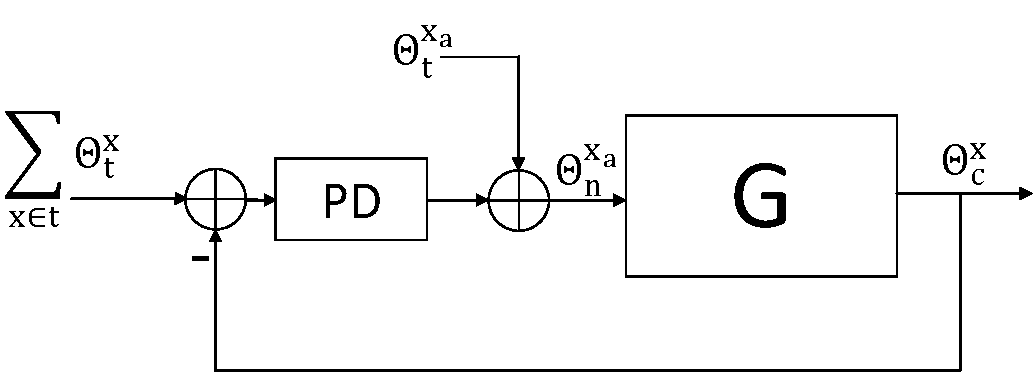
\includegraphics[width=0.8\columnwidth]{./pix/blockDiagram3.pdf}
  \caption{Block diagram of the balance controller used to balance Hubo in this work.}
  \label{fig:ctrlBlockDiagram}
\end{figure}

The control law is as follows
%ffFor the ankle roll (in the coronal plane) it is always assumed that the desired orientation of the COM is zero degrees.  Thus the roll of the IMU is taken as the error.

\begin{equation}
\theta_n^{x_a} = \theta_t^{x_a} + \left(K_p^x+sK_d^x\right)\left(\sum\limits_{x \in t} \theta_{t}^x - \theta_{c}^x\right)
%\theta_{n}^x = \theta_{t}^x + \left(K_p^x+sK_d^x\right)\left(\sum \theta_{t}^x - \theta_{c}^x\right)
%\theta_{n}^x = \theta_{t}^x + (K_p^x+sK_d^x)(\sum \theta_{t}^x - \theta_{c}^x)
%\theta_{new} = \theta_{traj} + (K_p+sK_d)(\sum \theta_{leg} - \theta_{IMU})
\end{equation}

Where $\theta_t$ is the desired trajectory of the lower body (pitch or roll), $x$ denotes pitch or roll and $x_a$ denotes pitch or roll on the ankle.  $\theta_{c}$ is the orientation of the center of mass in the global frame.  $\theta_n$ is the resulting trajectory.  $K_p$ and $K_d$ are the proportional and derivative gains.  The resulting control allows for a stable stance even with perturbations from upper body motions.



\section{Method Comparison}\label{sec:comparison}
All three methods described are stable during the throwing motion and can successfully throw a baseball.  Table~\ref{table:comp} shows the end-effector (EEF) velocity, joint failure rate, overhand or underhand throwing and stability of the three different methods of end-effector velocity control used in this paper human-robot joint mapping (MoCap), SRM based and key-frame.


\begin{small}
\begin{table}[!t]
%% increase table row spacing, adjust to taste
\renewcommand{\arraystretch}{1.3}
% if using array.sty, it might be a good idea to tweak the value of
% \extrarowheight as needed to properly center the text within the cells
\caption{Comparison between the three different methods of end-effector (EEF) velocity control: human-robot joint mapping (MoCap), SRM based and key-frame}
\label{table:comp}
\centering
\begin{tabular}{|c|c|c|c|c|}
\hline
  				& EEF 																	& Joint 						& Throw						& Stable  			\\
  				& Velocity ($\frac{m}{s}$)							& Failure (\%)			& Overhand (y/n)	& (y/n)					\\
\hline	
MoCap 		& 4.0																		& 0									& n								& y 						\\
\hline
SRM 			& 4.9																		& 10								& y								& y							\\
\hline
Key-Frame & 4.8 																	& 0 								& y								&	y							\\
\hline
\end{tabular}
\end{table}
\end{small}

The SRM technique worked well however the large jerk on each of the joints created large torques caused the motor controller to over torque/current and shutdown 10\% of the time.  
The pitch needs to work 100\% of the time thus this method is not well suited for the event.  
Both the human-robot joint mapping via MoCap and key-frame based methods consistently worked and stayed stable.  A secondary objective is to have the throwing motion be overhand like a standard Major League Baseball pitcher.  
Due to the constraints placed on the joint mapping of the MoCap method in Section~\ref{sec:sec:mocap} an over arm throw would be impossible to preform due to the robot's $\pm180^o$ joint limitations.  The key-frame method was chosen as the method to throw the ball.  Section~\ref{sec:finalDesign} describes the modifications to the system to allow it to reliably throw the pitch the desired distance.
The final goal is the have an end-effector velocity of 9.47 $\frac{m}{s}$ at $45^o$.  
The key-frame method was tested to throw at 4.8 $\frac{m}{s}$.  
To increase the end-effector velocity the upper body motion was kept unchanged but the lower body added a stepping motion with its legs.
The stepping motion consists of lifting the left foot up, pushing forward with the right and move the left forward 10 cm.  
Stepping with your non-dominant foot, and pushing with the dominant, when throwing overhand is common practice to increase the distance you can throw a ball.  
Jaemi Hubo throws with its right hand and steps with its left.  
This increased the end-effector velocity from 4.8 $\frac{m}{s}$ to 7.1 $\frac{m}{s}$.
Fig.~\ref{fig:hubo-step} shows the stepping motion of the robot.

\begin{figure}[t]
  \centering
\includegraphics[width=0.8\columnwidth]{./pix/throwPractice.png}
  \caption{Hubo stepping 10 cm up and forwards increasing the end effector velocity by 2.3 $\frac{m}{s}$.}
  \label{fig:hubo-step}
\end{figure}

The addition of pushing off with the right foot and stepping forward introduced two problems.  1) The ZMP criteria is not satisfied throughout the motion and 2) the right foot would slip when pushing its body forward.  
To avoid slip \textit{hook and loop} was paced on the bottom of the right foot (non-dominant) and on the throwing platform.  
This did not permanently attach the robot to the platform but it did allow for more friction between the foot and the ground.
This allowed the balancing controller to function adequately for the short step and maintain stability.
The platform was added to ensure a more consistent ground for the robot to balance on than the baseball field can inherently provide.

\begin{figure}[t]
  \centering
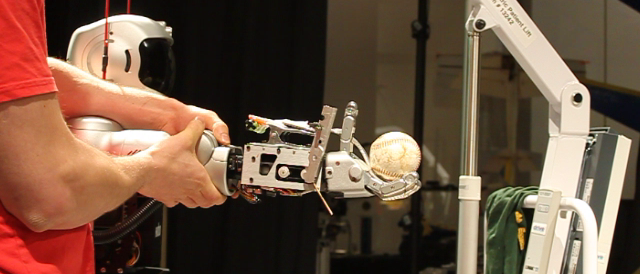
\includegraphics[width=0.4\columnwidth]{./pix/arm0.png}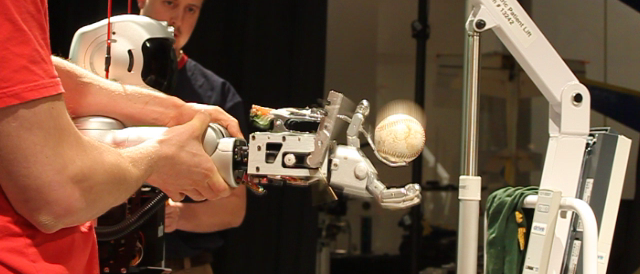
\includegraphics[width=0.4\columnwidth]{./pix/arm1.png}
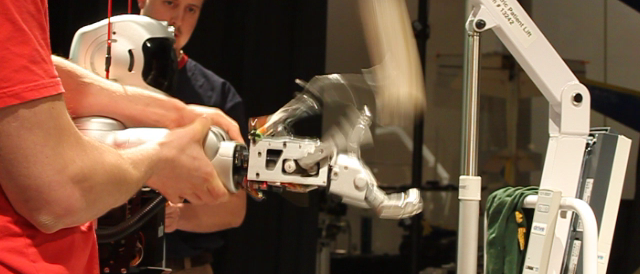
\includegraphics[width=0.4\columnwidth]{./pix/arm2.png}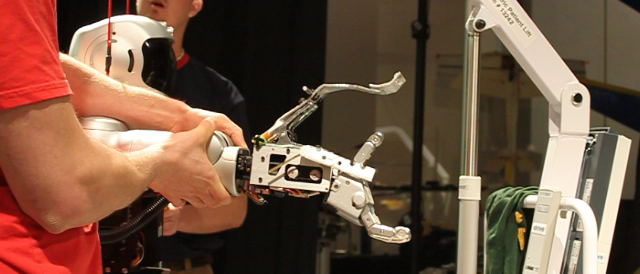
\includegraphics[width=0.4\columnwidth]{./pix/arm3.png}
%\includegraphics[width=1.0\columnwidth]{./pix/finalSpring1.png}
%\includegraphics[width=1.0\columnwidth]{./pix/finalSpring2.png}
%\includegraphics[width=1.0\columnwidth]{./pix/finalSpring3.png}
  \caption{Spring loaded mechanism test launching the baseball.  Top-Left: Pre-launch.  Top-Right/Bottom-Left: Launch.  Bottom-Right: Pos-launch.  The mechanism added 3.0 $\frac{m}{s}$ to the end-effector velocity at its release point.}
  \label{fig:hubo-spring}
\end{figure}

\begin{figure}[t]
  \centering
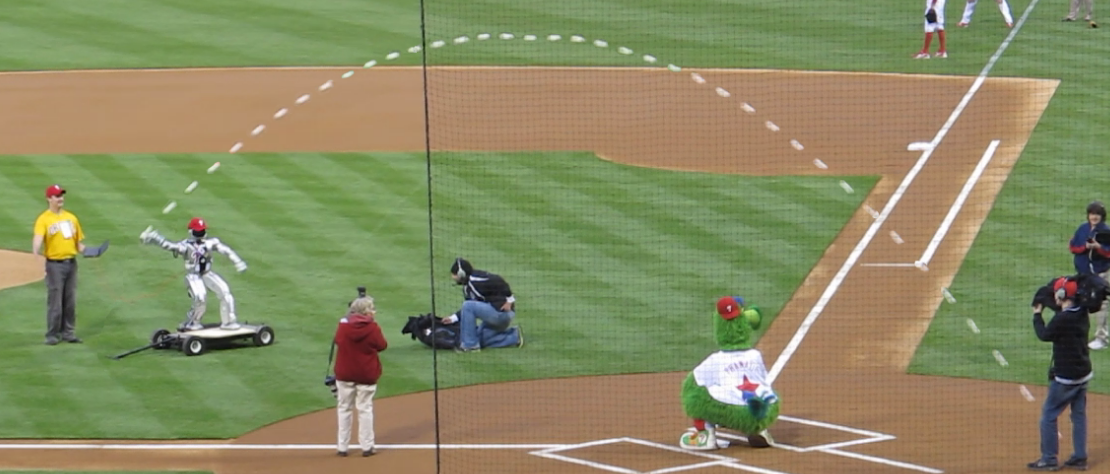
\includegraphics[width=1.0\textwidth]{./pix/philliesThrow.png}\\
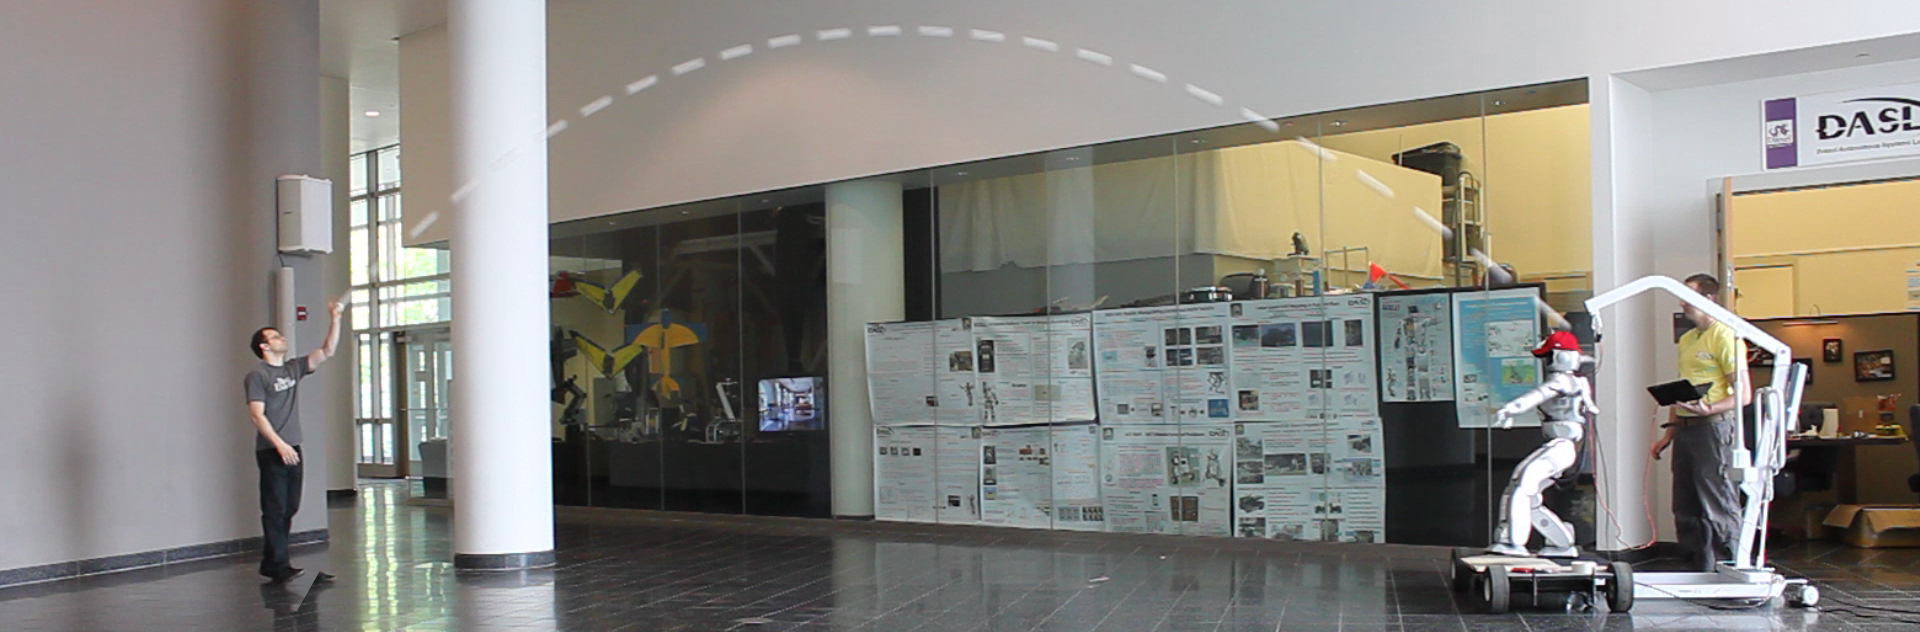
\includegraphics[width=1.0\textwidth]{./pix/preThrow2.png}
  \caption{(TOP) Pitch at Phillies Game.  (BOTTOM) Practice pitch at Drexel.  Frame overlay of the Hubo throwing overhand a distance of 10 m (32.8 feet) with a release angle of 40$^o$ and a tip speed of 10 $\frac{m}{s}$.  Captured at 20 fps with a shutter speed of 1/30 sec.  Each of the white dashes of in the image is the actual baseball as picked up by the video camera.}
  \label{fig:hubo-throw-test}
\end{figure}

An additional 2.5 $\frac{m}{s}$ was needed to give a proper throw.  
Borrowing from the GRASP Lab and their high powered pneumatic wrist on their PhillieBot, a spring loaded mechanism was added to Hubo's wrist, see Fig.~\ref{fig:hubo-spring}.
The addition of this mechanism allowed the robot to achieve an end-effector velocity magnitude of 10 $\frac{m}{s}$.
Fig.~\ref{fig:hubo-throw-test} shows a frame overlay of the the Hubo throwing a regulation baseball 10 m (32.8 feet).
Fig.~\ref{fig:hubo-throw} shows the same throw at Citizens Bank Park on April $28^{th}$, 2012.






\section{CONCLUSION AND FUTURE WORK}\label{sec:conc}

As the results in Fig.~\ref{fig:sparseRegion} in Section~\ref{sec:reslts} show the approach presented in this paper was successful for underhand throwing.  This approach also preforms overhand throwing if the velocity direction, duration, and magnitude falls within the SRM.  While not presented in this paper, results of overhand throwing will be presented in future dissemination of this work.  This work is also constructed in such a way that it is easily applicable to other low and high DOF robots.

The paper described a solution that coincides with our future efforts.  The next logical step is to incorporate full body motion and balancing to the velocity trajectory calculations to further advance the overarching goal of full body end-effector velocity control.

%In the end we solved the problem in the direction that we are going in.  The next logical step is to incorporate full body motion and balancing to the velocity trajectory calculations to further advance us towards our overarching goal.


%This work has shown a valid method of creating trajectories to achieve end-effector velocity control for high degree of freedom position controlled robots.  It was shown the full reachable area does not need to be known to achieve the desired velocity if a good collision model of the robot is available.  It was found that the limiting factor was the robot's physical joints.  This system does create trajectories that fall within the actuators' limitations, however this is not guaranteed.  Immediate future work includes creating a system that will guarantee actuator compliance with the generated trajectory.


% An example of a floating figure using the graphicx package.
% Note that \label must occur AFTER (or within) \caption.
% For figures, \caption should occur after the \includegraphics.
% Note that IEEEtran v1.7 and later has special internal code that
% is designed to preserve the operation of \label within \caption
% even when the captionsoff option is in effect. However, because
% of issues like this, it may be the safest practice to put all your
% \label just after \caption rather than within \caption{}.
%
% Reminder: the "draftcls" or "draftclsnofoot", not "draft", class
% option should be used if it is desired that the figures are to be
% displayed while in draft mode.
%
%\begin{figure}[!t]
%\centering
%\includegraphics[width=2.5in]{myfigure}
% where an .eps filename suffix will be assumed under latex, 
% and a .pdf suffix will be assumed for pdflatex; or what has been declared
% via \DeclareGraphicsExtensions.
%\caption{Simulation Results}
%\label{fig_sim}
%\end{figure}

% Note that IEEE typically puts floats only at the top, even when this
% results in a large percentage of a column being occupied by floats.


% An example of a double column floating figure using two subfigures.
% (The subfig.sty package must be loaded for this to work.)
% The subfigure \label commands are set within each subfloat command, the
% \label for the overall figure must come after \caption.
% \hfil must be used as a separator to get equal spacing.
% The subfigure.sty package works much the same way, except \subfigure is
% used instead of \subfloat.
%
%\begin{figure*}[!t]
%\centerline{\subfloat[Case I]\includegraphics[width=2.5in]{subfigcase1}%
%\label{fig_first_case}}
%\hfil
%\subfloat[Case II]{\includegraphics[width=2.5in]{subfigcase2}%
%\label{fig_second_case}}}
%\caption{Simulation results}
%\label{fig_sim}
%\end{figure*}
%
% Note that often IEEE papers with subfigures do not employ subfigure
% captions (using the optional argument to \subfloat), but instead will
% reference/describe all of them (a), (b), etc., within the main caption.


% An example of a floating table. Note that, for IEEE style tables, the 
% \caption command should come BEFORE the table. Table text will default to
% \footnotesize as IEEE normally uses this smaller font for tables.
% The \label must come after \caption as always.
%
%\begin{table}[!t]
%% increase table row spacing, adjust to taste
%\renewcommand{\arraystretch}{1.3}
% if using array.sty, it might be a good idea to tweak the value of
% \extrarowheight as needed to properly center the text within the cells
%\caption{An Example of a Table}
%\label{table_example}
%\centering
%% Some packages, such as MDW tools, offer better commands for making tables
%% than the plain LaTeX2e tabular whffich is used here.
%\begin{tabular}{|c||c|}
%\hline
%One & Two\\
%\hline
%Three & Four\\
%\hline
%\end{tabular}
%\end{table}


% Note that IEEE does not put floats in the very first column - or typically
% anywhere on the first page for that matter. Also, in-text middle ("here")
% positioning is not used. Most IEEE journals/conferences use top floats
% exclusively. Note that, LaTeX2e, unlike IEEE journals/conferences, places
% footnotes above bottom floats. This can be corrected via the \fnbelowfloat
% command of the stfloats package.







% conference papers do not normally have an appendix


% use section* for acknowledgement
\section*{Acknowledgment}

This project was conducted by the Drexel Autonomous Systems Lab (DASL), the Music Entertainment Technology Lab (MET)\footnote{Music Entertainment Technology Lab: http://music.ece.drexel.edu}.
support was provided by a Partnerships for International Research and Education (PIRE) \#0730206, and Major Research Infrastructure Recovery and Reinvestment (MIRR) \#CNS-0960061 sponsored by the the U.S. National Science Foundation (NSF).
Special thanks for organization and technical assistance goes to the Philadelphia Science Festival, Robert Ellenberg and Roy Gross.  
The robot platform used was Hubo, designed and created by our partner Dr. Jun-Ho Oh, Department of Mechanical Engineering, Korean Advanced Institute of Science and Technology, Daejeon, South Korea.% <-this %





% trigger a \newpage just before the given reference
% number - used to balance the columns on the last page
% adjust value as needed - may need to be readjusted if
% the document is modified later
%\IEEEtriggeratref{8}
% The "triggered" command can be changed if desired:
%\IEEEtriggercmd{\enlargethispage{-5in}}

% references section

% can use a bibliography generated by BibTeX as a .bbl file
% BibTeX documentation can be easily obtained at:
% http://www.ctan.org/tex-archive/biblio/bibtex/contrib/doc/
% The IEEEtran BibTeX style support page is at:
% http://www.michaelshell.org/tex/ieeetran/bibtex/
%\bibliographystyle{IEEEtran}
% argument is your BibTeX string definitions and bibliography database(s)
%\bibliography{IEEEabrv,../bib/paper}
%
% <OR> manually copy in the resultant .bbl file
% set second argument of \begin to the number of references
% (used to reserve space for the reference number labels box)
%\begin{thebibliography}{1}


\linespread{0.8}

\bibliographystyle{IEEEtran}
%\bibliographystyle{plain}
\bibliography{throwing}{}
  
%\end{thebibliography}




% that's all folks
\end{document}


